\chapter{Medium voltage electrical system}

	\section{Beacon circuits}
	\paragraph{} In series circuit is selected for beacon circuits, illustrated in figure \ref{series}. This option is chosen because its advantages.
	\begin{figure}[H]
		\centering
		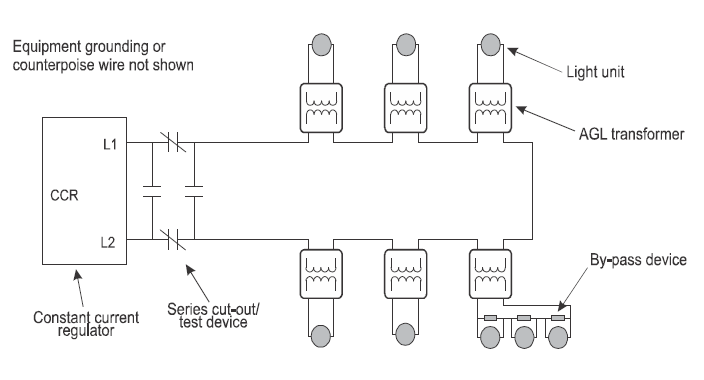
\includegraphics[clip, trim=0cm 0cm 0cm 0cm, width=0.7\textwidth]{./images/electric/series}
		\caption{Series lighting circuit.}
		\label{series}
	\end{figure}

	The constant current regulators of a series circuit, maintain a constant current independent of the load on the circuit. Thus, the same current will flow in a long circuit as in a shorter circuit and will remain the same even if some of the lamps fail. A short circuit across the output of a constant current regulator is a no-load condition and an open circuit is an overload. In a simple direct-connected series circuit, a lamp failure causes an open circuit; hence, it is necessary to provide an aerodrome ground lighting (AGL) transformer, as part of the circuit design, to maintain continuity of the circuit with lamp failure. Where a single transformer is used to supply several light units, as shown in Figure \ref{series}, a by-pass device is incorporated to ensure continuity on the secondary side.
	
	\subsection{Interleaving}
	\paragraph{} As a further means of assuring availability in case of failure, arrangement is made to enable switching to a spare regulator, as shown in Figure \ref{interleaved}. This method may be used where the regulator consists of the regulating component and input/output transformers. In the case of regulators that consist of only the regulating component, a rack mounted or plug-in design is used and availability is achieved by use of a spare regulator, Figure \ref{spare}, that can be readily installed in
	place of the failed regulator.
	
	\begin{figure}[H]
		\centering
		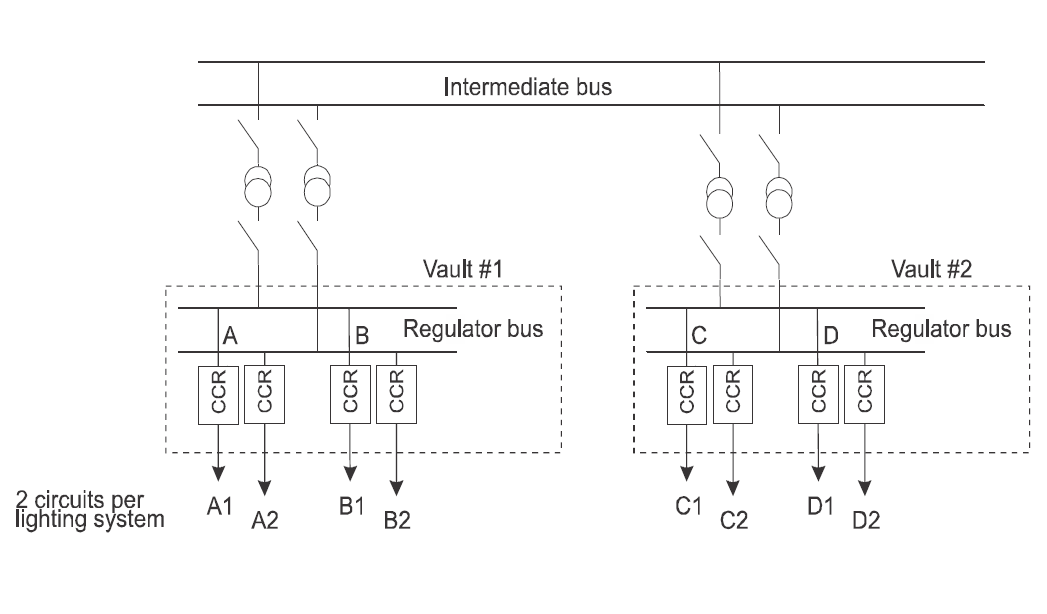
\includegraphics[clip, trim=0cm 0cm 0cm 0cm, width=0.8\textwidth]{./images/electric/interleaved}
		\caption{Provision of interleaved circuits.}
		\label{interleaved}
	\end{figure}

	\begin{figure}[H]
		\centering
		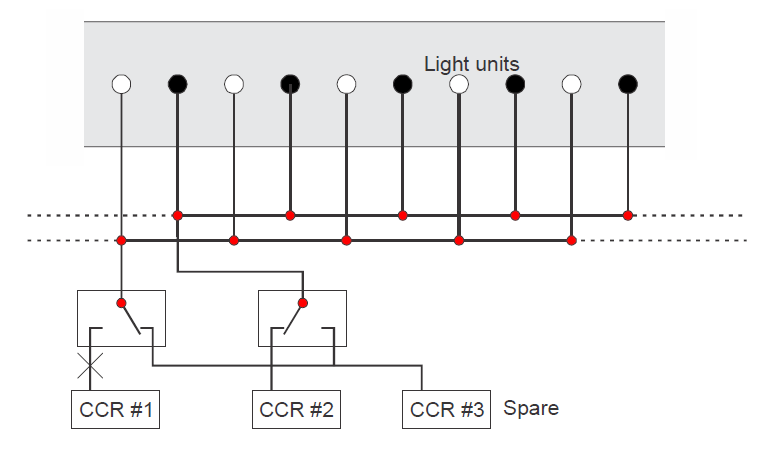
\includegraphics[clip, trim=0cm 0cm 0cm 0cm, width=0.7\textwidth]{./images/electric/spare}
		\caption{Use of a spare regulator.}
		\label{spare}
	\end{figure}
	
	
		\subsection{Runway centreline and touchdown lighting systems}
		\paragraph{} Annex 14, Volume I, requires that runway centreline lights show variable white to a distance of 900 m from the threshold, then alternating variable white and red from 900 m (or from the mid-point of the runway) to 300 m from the runway end after which only red is shown to the pilot. Figure \ref{rnwCentre} illustrates the interleaving for the first white only portion of the system. Similar interleaving would be used for the final all red portion.		
		
		\begin{figure}[H]
			\centering
			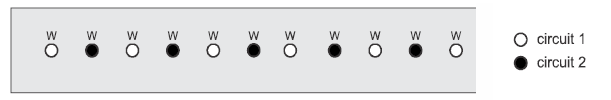
\includegraphics[clip, trim=0cm 0cm 0cm 0cm, width=0.7\textwidth]{./images/electric/rnwCentre}
			\caption{Runway centreline.}
			\label{rnwCentre}
		\end{figure}
		
		Interleaving to preserve spacing, Figure \ref{spacing}, is selected for the coded white/red portion of the system. This configuration, does not preserve the coding (with circuit failure the lights are either all red or all white), but does maintain an acceptable spacing for provision of a pattern of lights for centreline guidance (the spacing is doubled with circuit failure).
		
		\begin{figure}[H]
			\centering
			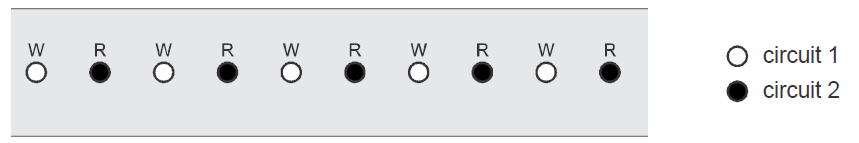
\includegraphics[clip, trim=0cm 0cm 0cm 0cm, width=0.7\textwidth]{./images/electric/spacing}
			\caption{Interleaving to preserve spacing.}
			\label{spacing}
		\end{figure}
	
		Figure \ref{touchdown} also illustrates the interleaving of runway touchdown zone lights. In this case three circuits will be used to preserve longitudinal spacing in case of one circuit failure.	
		\begin{figure}[H]
			\centering
			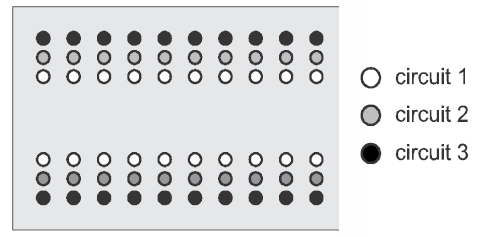
\includegraphics[clip, trim=0cm 0cm 0cm 0cm, width=0.7\textwidth]{./images/electric/touchdown}
			\caption{Interleaving by horizontal lines with three circuits.}
			\label{touchdown}
		\end{figure}
		
		
		\subsection{Taxiway centreline lighting system}
		\paragraph{} Taxiway centreline lighting circuits will be interleaved on those parts of the taxiway system that are considered as essential in category II/III conditions but, for economic reasons, a single circuit may be used for other taxiways.
		
		Three circuits for interleaving procedure will be use, figure \ref{inter3}. Because there is a lot of operations movement, is essential to preserve both spacing and colour, to reduce the chance of pilots getting lost.
		
		\begin{figure}[H]
			\centering
			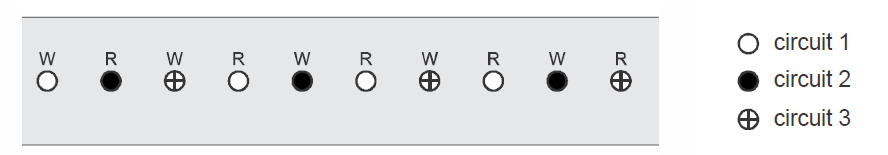
\includegraphics[clip, trim=0cm 0cm 0cm 0cm, width=0.7\textwidth]{./images/electric/inter3}
			\caption{Interleaving to preserve both spacing and colour.}
			\label{inter3}
		\end{figure}
		
		\subsection{Stop bar electrical circuit}
		\paragraph{} Stop bars will be controlled independently of each other and of the taxiway centreline lights. The electrical circuits will be interleaved so that all of the lights of a stop bar will not fail at the same time.
		
		\subsection{Approach lighting system}
		
			\subsubsection{Visual approach, PAPI electrical circuit}
			\paragraph{} Visual approach slope indicator systems will have two circuits per runway end because they are operated with an ILS system.
			
			A full PAPI or T-VASI will be installed on both sides of the runway, the power to all light units on one side of the runway will be supplied by the same circuit. This arrangement ensures that should one circuit fail a complete pattern will be retained on the other side of the runway.
					
			
			\subsubsection{Precision approach}
			\paragraph{} Precision approach interleaving implemented are summarized on figure \ref{pApp}.
			\begin{figure}[H]
				\centering
				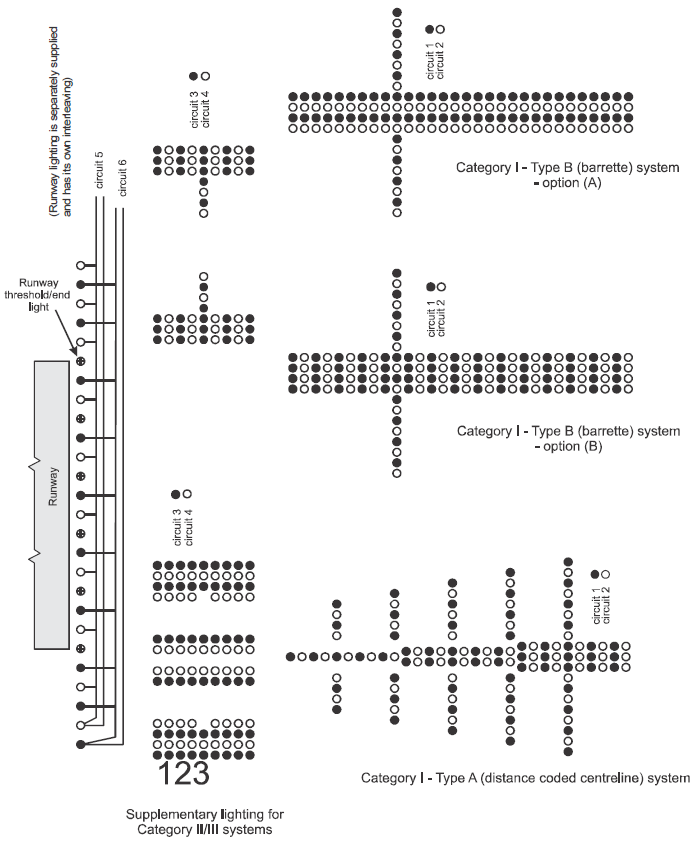
\includegraphics[clip, trim=0cm 0cm 0cm 0cm, width=0.8\textwidth]{./images/electric/pApp}
				\caption{Precision approach lighting system interleaving.}
				\label{pApp}
			\end{figure}
			
		\subsection{Runway holding position signs}
		\paragraph{} Runway holding position signs will be installed such that separate circuits are used for the signs on each side of the taxiway.
		
		\subsection{RETIL electrical circuit}
		\paragraph{} The rapid exit taxiway indicator lights (RETIL) system is composed of a pattern of in-pavement fixtures used to indicate the approach to a runway exit. In as much as the system has a small quantity of fixtures and each is necessary for the distance coding, the RETIL system is not provided with interleaving but has a single circuit that is fed from a separate constant current regulator.
		
		Failure of one light within a barrette results in a malfunction of the system. Therefore, the system will be provided with an automatically turn off the entire system circuit, if there is a loss of a single light unit.
				
		
	\section{Constant current regulators}
	\paragraph{} The electrical power for the aerodrome ground lighting circuits (series circuit) is supplied by constant current regulators (CCRs) because this facilitates constant light output over long distances, as is the case for aerodrome runways. The regulators are designed to produce a constant current output that is independent of variations in the circuit load and input voltage of the power source. They are also designed to provide two or more output currents when
	dimming of the lights is required. 
	
	Projected airport will have two CCRs in order to power the aerodrome ground lighting circuit. Each one, powers the lights of half of each runway.
	
	
	\section{Wire channelling}
	\paragraph{} Primary beaconing 5KV grid and low tension circuit will be installed in  ducts encased in concrete, figure \ref{concrete}. All ducts installed in concrete encasement will be placed on a layer of concrete not less than 75 mm thick.
	
	Flared ends of ducts or couplings will be installed flush with the concrete encasement or inside walls of manholes or handholes. Interlock spacers will be used at not more than 1.5 m spacing to ensure uniform spacing between ducts. Joints in adjacent ducts will be staggered a minimum of 600 mm apart and will be made waterproof prior to concreting. Concrete-encased duct will be installed so that the top of the concrete envelope or conduit is not less than 450 mm below the stabilized base course where it is installed under roadways, railroads, runways, taxiways, other paved areas and ditches, and not less than 450 mm below the finished grade elsewhere. Counterpoise wires are provided as required.
	
	\begin{figure}[H]
		\centering
		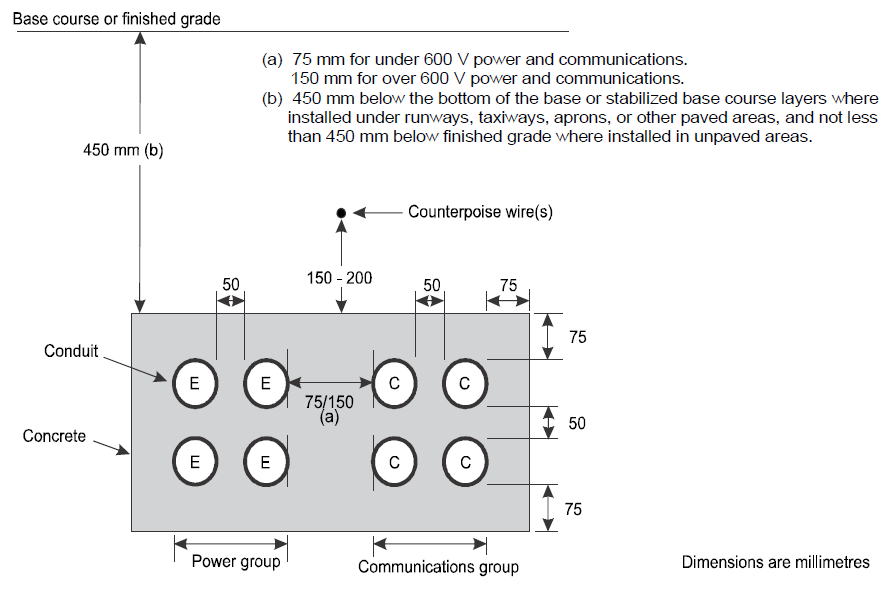
\includegraphics[clip, trim=0cm 0cm 0cm 0cm, width=\textwidth]{./images/electric/concrete}
		\caption{Concrete encased duct bank.}
		\label{concrete}
	\end{figure}
	
	In order to make easier the maintenance and installation, these connections will be simple and when possible in straight lines. When there is a change in direction, a manhole or hand-hole will be installed.
	
	
